\chapter{Algoritmul de repartizare}

Problema pe care își propune această aplicație să o rezolve este o instanță a problemei asignării sau problema atribuirii (\textit{assignment problem}). Este de precizat că cele două nume vor fi folosite interschimbabil în secțiunile următoare. În cazul de față, instanța este reprezentată de o mulțime de studenți, fiecare cu o ordonare a unor prefereințe, și o mulțime a propunerilor profesorilor (proiecte sau tematici generale). Cerința este reapartizarea optimă a propunerilor către studenți în funcție de preferințele acestora.

În literatura de specialitatea au fost descriși și dezvoltați diverși algoritmi de rezolvare a unei astfel de instanțe a problemei atribuirii. Algoritmul implementat de aplicația \thesistitle{} este unul din clasa de algoritmi de licitație (\textit{auction algorithms}), descris în lucrarea "Assignment Problem with Constraints" scrisă de către Ulrich Bauer, Facultatea de Informatică a Universității Tehcnice din München, 2005. Pentru a descrie coerent și cât mai clar logica acestui algoritm, în secțiunile următoare vor fi descrise problema atribuirii și similitudinile acesteia cu o problemă de flux, conceptele matematice ale algoritmilor propuși pentru rezolvare și pașii algoritmului implementat pentru instanța prezentă.

\section{Problema asignării (atribuirii)}

Problema simetrică a asignării constă în două mulțimi $X$ și $Y$ de dimensiuni egale, o mulțime $E \subseteq X \times Y$ și o funcție de cost $c_{xy}$ pentru oricare pereche posibilă $(x, y) \in E$. Scopul este cuplarea oricărui element din $X$ cu un element din $Y$ ca la final costul total să fie minim \cite{assignment}.

În contextul grafurilor, această problemă poate fi redusă la problema fluxului de cost minim într-un  graf bipartit $G=((X \bigcup Y,\ E)$ cu o funcție de cost $c_{xy},\ (x, y) \in E$, și capacitatea $u_xy = 1, \forall (x, y) \in E$. 

Expresia matematică a problemei \cite[p.~6]{assignment} este 
\[ minimizarea \sum_{(i, j) \in E} c_{ij} x_{ij} \]
astfel încât
\[ \sum_{j:(i, j) \in E} x_{ij} = 1, \forall i \in X, \]
\[ \sum_{i:(i, j) \in E} x_{ij} = 1, \forall j \in Y, \]
\[ x_{ij} \geq 0, \forall (i, j) \in E \].

Variabila $x_{ij}$ indică câtă unități de flux sunt trimise pe muchia $(i, j)$.

Cu toate acestea, problema repartizării fiecărui student o teză de licență în funcție de preferințele sale este o problemă asimetrică deoarece numărul de propuneri, $|Y|$, este mai mare sau egal decât numărul de studenți (trebuie să fie măcar egal pentru a putea atribui fiecărui student o lucrare). La final, o soluția determinată se va afla în variabila $x_{ij}$ unde dacă $x_{ij} = 1$, atunci studentului $i$ îi este repartizată propunerea $j$ din totalul de propuneri al tuturor profesorilor.

Important de precizat este că în acest caz, rating-ul total al preferințelor satisfăcute trebuie maximizat. De aceea, este realizată o normalizare în primă instanță pentru a transforma rating-urile în costuri, prin calcularea $c_{ij} = 101 - rating_{ij},\: rating_{ij} \in \mathbb{N} \cap [1, 100],\: \forall (i, j) \in E$.

\section{Algoritmul de licitație}

Algoritmul de licitație este o metodă intuitivă ce rezolvă problema clasică a atribuirii (asignării), reușind de asemenea să depășească în performanță algoritmi similari, fiind în același timp potrivit pentru calculul în paralel \cite[p.~1]{auction}. Acest algoritm a fost propus de matematicianul Dimitri Bertsekas și este în sine o metodă euristică aplicată algoritmului \textit{push/relabel} pentru a îmbunătăți rezultatele practice \cite[p.~24]{assignment}, având în mod similar o complexitate de $\mathcal{O}(n m \log(n C))$ unde $n$ este numărul total de noduri ($|X|+|Y|$), $m$ este numărul de muchii $|E|E$, iar $C = max_{(i, j)}\{c_{ij}\}$ este maximul costurilor. 

Algoritmul de licitație poate fi descris ca o licitație în viața reală. Elementele din mulțimea $X$, studenții, licitează pentru elementele din $Y$, lucrările propuse de profesori. Pentru un student $i$, propunerea $j$ este cea mai benfică dacă suma costului $c_{ij}$ și prețul $\pi(j)$ este minim, iar o propunere este atribuită studentului cu cea mai bună ofertă\cite{assignment}. Funcția $\pi$ este utilizată în pasul de reetichetare (\textit{relabel}) a unei propuneri.

Pentru a permite finalizarea algoritmului, prețurile $\pi$ trebuie să crească cu o valoare $\epsilon$. Mai mult decât atât, Bertsekas a fost primul care a propus scalarea prin $\epsilon$ (\textit{$\epsilon$-scaling}) pentru a îmbunătăți performanța algoritmului în cazul instanțelor unde numărul de obiecte din $Y$ licitate este mai mic. În cazul în care $\epsilon$ este prea mic, poate apărea un "război al prețurilor" când este nevoie de o creștere mai substanțială a prețurilor, deci un număr mare de iterații, până anumiți studenți găsesc propuneri mai profitabile decât cele licitate. Soluția este execuția algoritmului începând cu $\epsilon$ inițializat cu cel mai mare cost al preferințelor ($C$) și scădereaa treptată a acestuia de la o iterație la alta.

Algoritmul de licitație poate fi corelat cu unul de calculare a unui flux de cost minim, cu un graf $G=(X \cup Y, E)$ unde $X$ reprezintă studenții, iar $Y$ propunerile. Este definită o nouă variabilă 
$c_{ij}^\pi$ numită costul redus al muchiei $(i, j)$ din graful $G=(V, E)$ în raport cu funcția de preț $\pi: V \rightarrow \mathbb{R}_+$,\; $c_{ij}^\pi = c_{ij} - \pi(i) + \pi(j)$.

Un pas de licitație este numit \textit{double-push} deoarece este echivalent cu operațiile \textit{push} și \textit{relabel}. Când un student $x$ licitează pentru un proiect $y$, este efectuat un flux pe muchia $(x, y)$. Dacă $y$ a fost deja asigant unui $x'$, $y$ transmite flux către $x'$ deoarece are un exces pozitiv.

\subsection{Algoritmul de licitație pentru problema asimetrică a asignării}

În cazul problemei asimetrice de asignare, $|X| \leq |Y|$ și trebuie determinat care dintre muchii trebuie luate în calcul. Se poate întâmpla ca după o iterație, prețul unui element din $Y$ poate deveni prea mare și poate rămâne neasignat în iterația următoare, deși ar putea fi preferat de către un student. În cazul problemei simetrice, fiecare $y \in Y$ este asignat.

O primă abordare este transformarea problemei asimetrice într-una simetrică prin introducerea unor $|Y| - |X|$ noduri "virtuale" în mulțimea $X$, fiecare dintre ele conectat la toate nodurile din $Y$  cu câte un cost 0. Acest lucru poate rezulta însă la un graf dens din punct de vedere al muchiilor.

O altă abordare, utilizată și în proiectul de față, este utilizarea unui arbore binar (\textit{binary heap}). De fiecare dată când este reetichetat (\textit{relabeled}) un nod care nu se află în heap, este introdus în heap și eliminat din acesta nodul cu cel mai mic preț. Dacă acest nod este atribuit, fluxul pe muchia respectivă devine 0. Utilizând un arbore binar, reetichetarea nodului are loc cu o complexitate de $\mathbb{O}(\log(|X|)$, iar accesarea nodului cu cel mai mic preț este imediată deoarece se află în vârf. Complexitatea generală a algoritmului crește la $\mathbb{O}(n m \log(n C) \log(|X|))$, care nu afectează mult însă performanța algoritmului.

\section{Pseudocod}

Algoritmii următori scriși în pseudocod și utilizați de aplicație au fost descriși în lucrarea menționată anterior, \textit{Constrained Assignment} \cite{assignment}.

\subsection{Funcția \textit{doublePush} cu arbore binar (heap)}

\begin{algorithm}
	\caption{$doublePush(i)$}
	\begin{algorithmic}[1]
		\State Fie $(i, j)$ și $(i, k)$ muchii astfel încât $c_{ij}^\pi$ să fie minim și $c_{ik}^\pi$ al doilea cel mai mic
		\State $x_{ij} \gets 1$ //push 
		\If{$j \notin H$} // $H$ este arborele binar (heap)
			\State $H.put(\pi(j),\ j)$ //j este introdus în heap cu cheia prețul său actual
			\If{$|X| > H.size()$}
				\State $g \gets H.min()$
				\State $H.removeMin()$
				\If{$\exists f \in X$, $x_{fg} = 1$} //propunerea g este deja asignată unui student f
					\State $x_{fg} \gets 0$ //push
				\EndIf
			\EndIf
		\EndIf
		\If{$\exists h \in X$, $h \neq i$ și $x_{hj} = 1$} //propunerea j era deja atribuită unui alt student h
			\State $x_{hj} \gets 0$ //push
		\EndIf
		\State $\pi(j) \gets \pi(k) + c_{ik} - c_{ij} + \epsilon$ //relabel
	\end{algorithmic}
\end{algorithm}

\subsection{Funcția \textit{refine} de îmbunătățire a rezultatului}

\begin{algorithm}
	\caption{$refine()$}
	\begin{algorithmic}[1]
		\State $\epsilon \gets \epsilon / \alpha$ //$\alpha$ este o constantă aleasă în mod euristic
		\ForAll{$(i, j) \in E$}
			\State $x_{ij} \gets 0$
		\EndFor
		\While{$\exists i \in X$, $i$ neasignat}
			\State $doublePush(i)$
		\EndWhile
	\end{algorithmic}
\end{algorithm}

\subsection{Algoritmul de licitație pentru asignare}

\begin{algorithm}
	\caption{$solve()$}
	\begin{algorithmic}[1]
		\State $\epsilon \gets max_{(i, j) \in E}\{c_{ij}\}$
		\ForAll{$j \in Y$} //inițializează prețul tuturor propunerilor cu 0
			\State $\pi(j) \gets 0$
		\EndFor
		\While{$\epsilon \geq 1 / n$}
			\State $refine()$
		\EndWhile
		\State return $x$
	\end{algorithmic}
\end{algorithm}

\section{Implementare}

Implementarea algoritmului prezentat anterior a avut loc în limbajul Java pentru a putea fi folosit în cadrul unei aplicații de Spring Boot. A fost creată în mod special clasa \textit{Edge} pentru a modela muchiile dintre cele două mulțimi $X$ a studenților și $Y$ a propunerilor, mai precis preferințele studenților. Câmpul \textbf{start} indică indicele studentului și câmpul \textbf{end} indică indicele propunerii preferate.

\begin{figure}[H]
	\centering
	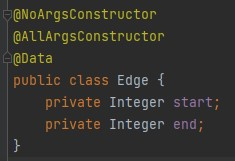
\includegraphics[width=0.5\textwidth, center]{edge-class.jpg}
	\caption{Clasa Edge}
\end{figure}

\subsection{Preprocesarea datelor}

Înainte de efectuarea algoritmului, este nevoie de operații de preprocesare pentru a converti obiectele primite de la baza de date (studenții, propunerile, preferințele) în variabile de input adecvate. Pentru acest lucru a fost creată clasa \textit{Convertor} care utilizează patru servicii, \texttt{accordService}, \texttt{preferenceService}, \texttt{proposalService} și \texttt{userService}, pentru a accesa înregistrările din baza de date, reținându-se în două liste \texttt{studIds} și \texttt{propIds} id-urile studenților (students) și propunerilor (proposals). Sunt eliminate id-urile care se află într-un acorduri acceptate, adică cele care au câmpul $\texttt{isAccepted} = true$.

Algoritmul este nevoit să primească listele $X$ și $Y$ sub formă de indecși ale elementelor în listele \texttt{studIds} \texttt{propIds}, iar nu id-urile în mod direct, deoarece propunerile pot fi de două feluri: proiect (project) sau tematică (topic). Tematicile pot avea un număr de locuri disponibile mai mare de 1, de aceea în \texttt{propIds} se adaugă duplicate ale aceluiași id câte locuri sunt disponibile.

Indecșii id-urilor studenților sunt reținute într-o variabilă \texttt{studIndices} de tipul \texttt{HashMap<Long, Integer>} unde cheile sunt id-urile, iar valorile sunt indecșii în lista de id-uri. Similar, indecșii propunerilor sunt reținuții în variabila \texttt{propIndices} de tipul \texttt{HashMap<Long, List<Integer>>} de această dată deoarece un id de propunere poate avea mai multe duplicate în listă.

După aceste convertiri, este calculată o variabilă $c$ a costurilor (similară modelului teoretic) de tipul \texttt{HashMap<Edge, Double>} unde cheile sunt muchiile (preferințele), iar valorile acestora sunt costurile. Un cost se calculează astfel: preferințele unui student sunt ordonate descrescător, teza de licență cea mai favorabilă primind costul 1.0, iar două propuneri cu același rating primind același cost.

\subsection{Algoritmul}

Algoritmul este modelat de clasa \textit{AssignAlgorithm} ce este inițializat cu variabilele $n$ numărul de studenți, $m$ numărul de propuneri, $c$ variabila costurilor. Clasa dispune de metodele similare algoritmilor prezentați anterior în pseudocod.

În metoda \textit{solve()} este inițializată o listă \texttt{unassigned} cu toți studenții neatribuiți. Se inițializează variabila $eps$ cu cel mai mare cost din $c$ și variabila $pi$ este setată pe valoarea 0 pentru toate propunerile. Cât timp $eps$ nu depășește pragul $alpha / (n + m)$ se execută metoda \textit{refine()}.

Metoda \textit{refine()} reinițializează variabila soluție $x$ cu 0 pe fiecare muchie. Se alege în mod aleatoriu un student neasignat și se execută metoda \textit{doublePushHeap(i)}.

\begin{figure}[H]
	\centering
	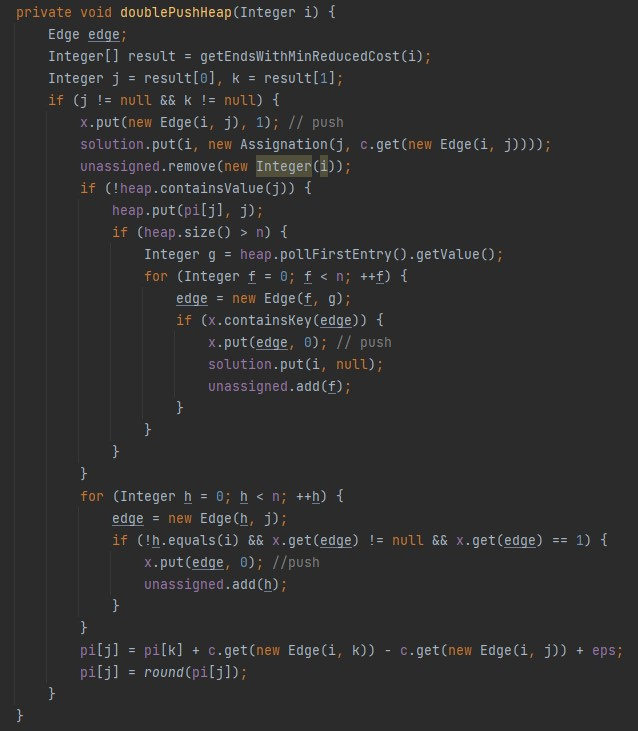
\includegraphics[width=0.7\textwidth, center]{double-push-method.jpg}
	\caption{Metoda \textit{doublePushHeap}}
\end{figure}

Este definită variabila locală \texttt{result} ca un tablou de două poziții. Poziția \texttt{result[0]} conține $j$, iar, \texttt{result[1]} conține $k$, unde $(i, j)$ este muchia cu cel mai mic cost redus și $(i, k)$ muchia cu al doilea cel mai mic cost redus. Variabila \texttt{heap} a fost declarată de tipul \texttt{TreeMap<Double, Integer>} unde cheile sunt prețurile propunerilor (\texttt{$\pi[j]$}) și valorile sunt indecșii. Acest lucru permite ordonarea propunerilor asignate în funcție de prețul acestora, de asemenea accesarea propunerii (elementului $j \in Y$) cu prețul $\pi(j)$ minim are loc în $\mathbb{O}(1)$.

Orice alt student $h$ asignat anterior propunerii $j$ este marcat ca fiind neasignat (push step). În contextul problemei fluxului într-un graf bipartit, fluxul dinspre studentul $i$ spre propunerea $j$ este setat pe 0.

\begin{figure}[H]
	\centering
	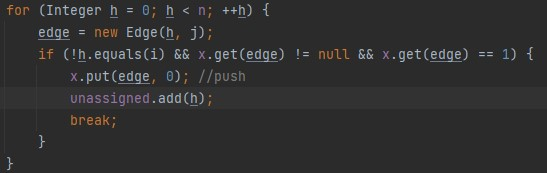
\includegraphics[width=1\textwidth, center]{push-step.jpg}
	\caption{Pasul de push}
\end{figure}

Pasul final este cel de reetichetare (relabel step) observat în imaginea următoare.

\begin{figure}[H]
	\centering
	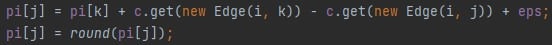
\includegraphics[width=1\textwidth, center]{relabel-step.jpg}
	\caption{Pasul de relabel}
\end{figure}

\subsection{Procesarea rezultatului}

Soluția constă într-o variabilă de tipul \texttt{Map<Integer, Assignation>} cu cheile reprezentând indecșii studenților în lista \texttt{studIds}. Valorile sunt de tipul \texttt{Assignation} ce conține câmpul \texttt{end} ce reprezintă indexul propunerii atribuite în lista \texttt{propIds} și câmpul \texttt{cost} ce are calculat calitatea preferinței satisfăcute. Acest lucru permite accesarea rapidă a soluției pentru un student $i$ și construirii rezultatului total.

\begin{figure}[H]
	\centering
	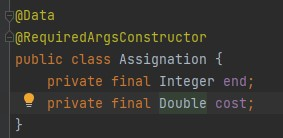
\includegraphics[width=0.6\textwidth, center]{assignation-type.jpg}
	\caption{Tipul Assignation}
\end{figure}

La finalul execuției algoritmului, există posibilitatea ca un număr de studenți să nu aibă proiecte atribuite în cazul în care aceștia nu au avut un număr de preferințe îndeajuns de mare. Dacă există o astfel de situație, se alege în mod aleatoriu un student dintre aceștia și îi este asignată o propunere dintre cele care nu au fost încă luate.

Rezultatul final este alcătuit în primul rând din studenții care au stabilit acorduri cu profesori pentru anumite proiecte, repartizările calculate de algoritm și repartizările ulterioare ale studenților neatribuiți.

Din punct de vedere tehnic, rezultatul transmis către front-end prin intermediul unui request de tipul GET este o listă de obiecte de tipul \texttt{MatchingDto} (DTO = Data Transfer Object).

\begin{figure}[H]
	\centering
	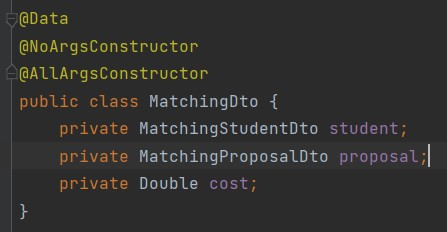
\includegraphics[width=0.7\textwidth, center]{matchingdto-class.jpg}
	\caption{Clasa MatchingDto}
\end{figure}

\begin{figure}
\centering
	\begin{minipage}{0.5\textwidth}
		\centering
		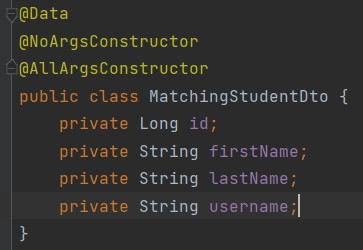
\includegraphics[width=1\linewidth]{matchingstudentdto-class.jpg}
		\caption{Clasa MatchingStudentDto}
	\end{minipage}%
	\begin{minipage}{0.5\textwidth}
		\centering
		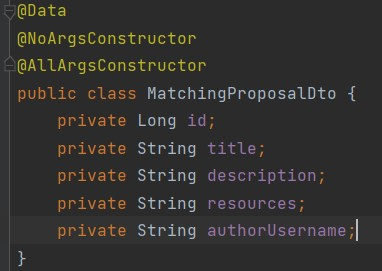
\includegraphics[width=1\linewidth]{matchingproposaldto-class.jpg}
		\caption{Clasa MatchingProposalDto}
	\end{minipage}
\end{figure}

\section{Precizări}

Variabila \texttt{pi} conține valori reale, dar a fost considerat că o precizie de două variabile este de ajuns pentru efectuarea algoritmului. Pentru trunchierea valorilor, a fost implementată o metodă statică \texttt{round(double value)} care aproximează superior prețurile calculate.

\begin{figure}[H]
	\centering
	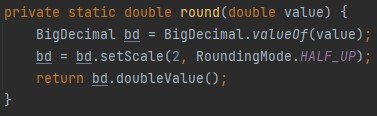
\includegraphics[width=1\textwidth, center]{round-method.jpg}
	\caption{Rotunjirea prețurilor}
\end{figure}

Constanta \texttt{alpha} a fost inițializată cu valoarea 10, urmând recomandările menționate în lucrarea \textit{Constrained Assignment} \cite[p.~46]{assignment}.

Variabila \texttt{eps} are valorea inițială egală cu cel mai mare cost dintre muchiile existente.
